\documentclass [a4paper,11pt]{article}
\usepackage{amssymb}
\usepackage{amsthm}
\usepackage[intlimits]{amsmath}
\usepackage[polish]{babel}
\usepackage[utf8]{inputenc}
\usepackage[T1]{fontenc}
\frenchspacing
\usepackage{indentfirst}
\usepackage{graphicx}
\usepackage{subfig}
\usepackage{mathptmx}
\usepackage{geometry}
\usepackage{wrapfig}
\usepackage{enumitem}
\usepackage{tabularx}

\title{Moduł Younga}
\author{Pęcak Tomasz, Bielech Maciej}

\begin{document}
	
	\renewcommand*{\figurename}{Rysunek} 
	\newgeometry{tmargin=2cm, bmargin=2cm, lmargin=2cm, rmargin=2cm}
	
	\linespread{1.5}
	\selectfont

	\begin{table}[]
		\centering
		\begin{tabular}{lllllll}
			\cline{1-6}
			\multicolumn{1}{|c|}{\begin{tabular}[c]{@{}c@{}}EAiIB\\ Informatyka\end{tabular}} & \multicolumn{2}{l|}{\begin{tabular}[c]{@{}l@{}}Pęcak Tomasz\\ Bielech Maciej\end{tabular}} & \multicolumn{1}{c|}{\begin{tabular}[c]{@{}c@{}}Rok\\ II\end{tabular}} & \multicolumn{1}{c|}{\begin{tabular}[c]{@{}c@{}}Grupa\\ 3a\end{tabular}} & \multicolumn{1}{c|}{\begin{tabular}[c]{@{}c@{}}Zespół\\ II\end{tabular}} &  \\ \cline{1-6}
			\multicolumn{1}{|c|}{\begin{tabular}[c]{@{}c@{}}Pracownia\\ FIZYCZNA\\ WFiIS AGH\end{tabular}} & \multicolumn{4}{l|}{\begin{tabular}[c]{@{}l@{}}Temat:\\ \textbf{Współczynnika załamania światła} \end{tabular}} & 
			\multicolumn{1}{l|}{\begin{tabular}[c]{@{}l@{}}nr ćwiczenia:\\ 51\end{tabular}} &  \\ \cline{1-6}
			\multicolumn{1}{|l|}{\begin{tabular}[c]{@{}c@{}}Data wykonania:\\ 25.11.2017\end{tabular}} & \multicolumn{1}{c|}{\begin{tabular}[c]{@{}c@{}}Data oddania:\\ 28.11.2017\end{tabular}} & \multicolumn{1}{l|}{\begin{tabular}[c]{@{}l@{}}Zwrot do poprawki:\\ \phantom{data poprawki}\end{tabular}} & \multicolumn{1}{l|}{\begin{tabular}[c]{@{}l@{}}Data oddania:\\  \phantom{data oddania}\end{tabular}} & \multicolumn{1}{l|}{\begin{tabular}[c]{@{}l@{}}Data zaliczenia:\\  \phantom{data zaliczenia}\end{tabular}} & \multicolumn{1}{l|}{\begin{tabular}[c]{@{}l@{}}OCENA:\\ \phantom{ocena}\end{tabular}} &  \\ \cline{1-6} 
		\end{tabular}
	\end{table}
	 \hspace{5mm}

	\section{Wstęp}
	Celem ćwiczenia było wyznaczenie wartości oporu pięciu różnych oporników oraz połączeń szeregowych, równoległych i mieszanych tych oporników.
	
	Aby określić wartości natężeń ($I$) prądów w obwodach elektrycznych używa się pierwszego prawa Kirchhoffa: 
	
	Dla węzła obwodu suma natężeń wpływających do tego węzła jest równa sumie natężeń wypływających z~niego. Jeśli przyjmiemy, że wartość natężenia prądów wypływających jest ujemna prawo to można zapisać w~następujący sposób: 
	\begin{equation}
		\label{eq:PPK}
		\sum_{x=1,2,...}I_x=0 \text{.}
	\end{equation}
	Do wyliczenia wartości napięć ($U$) na odbiornikach prądu w obwodzie zamkniętym służy drugie prawo Kirchhoffa:
	
	Suma napięć na wszystkich odbiornikach prądu jest równa sumie napięć na źródłach napięcia. Co można zapisać:
	\begin{equation}
	\label{eq:DPK}
	\sum_{i}U_i=\sum_{k}\epsilon_k \text{.}
	\end{equation}	
	Drugie prawo Kirchhoffa możemy zastosować jedynie, gdy obwód, dla którego stosujemy to prawo nie jest umieszczony w zmiennym polu magnetycznym.
	
	Do jednoznacznego znalezienia natężeń i napięć w obwodzie potrzebujemy współczynnika ich proporcjonalności. Tym współczynnikiem jest rezystancja ($R$). Tą proporcjonalność opisuje prawo Ohma:
	\begin{equation}
	\label{eq:PO}
	U=RI
	\end{equation}
	Mostek Wheatstone'a jest układem elektrycznym służącym do pomiaru rezystancji oporników. Schemat jego wykonania jest przedstawiony na rysunku (\ref{fig:mostek}).
	\begin{figure}[!h]
		\centering
		%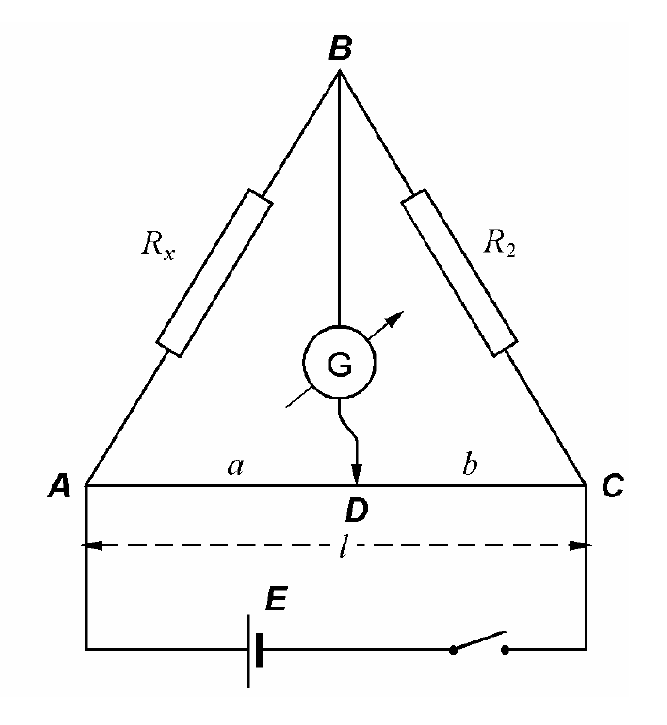
\includegraphics[width=0.6\textwidth]{mostek}
		\caption{Schemat mostka Wheatstone'a}
		\label{fig:mostek}
	\end{figure}

	Jest on utworzony poprzez połączenie czterech rezystorów ($R_x$ - rezystancja nieznana, $R_2$ - rezystancja opornicy dekadowej, $R_a$, $R_b$ - rezystancja odpowiednich części listwy z drutem oporowym), mikroamperomierza $G$ oraz źródła prądu $E$.
	
	Stosując prawa Kirchhoffa (\ref{eq:PPK} i \ref{eq:DPK}) i prawo Ohma (\ref{eq:PO}) dochodzimy do wzoru pozwalającego na wyznaczenie oporu nieznanego ($R_x$):
	\begin{equation}
	\label{eq:Mostek}
	R_x=R_2\frac{R_a}{R_b}\text{.}
	\end{equation}
	Korzystając z wzoru na opór właściwy, który jest wielkością charakteryzującą dany materiał (w tym przypadku drut o długości $AC$ ) i uwzględniając to, że drut jest drutem jednorodnym można wyznaczyć $R_a$ i $R_b$:
	\begin{equation}
	\label{eq:Opór Ra}
	R_a=\rho \frac{a}{S}\text{,}
	\end{equation}
	\begin{equation}
	\label{eq:Opór Rb}
	R_b=\rho \frac{b}{S}\text{,}
	\end{equation}
	gdzie $\rho$ to opór właściwy materiału, z którego wykonany jest drut, a $S$ to pole przekroju poprzecznego tego drutu. Uwzględniając te wzory w równaniu (\ref{eq:Mostek}) otrzymujemy zależność: 
	\begin{equation}
	\label{eq:Mostek2}
	R_x=R_2\frac{a}{b}\text{.}
	\end{equation}
	Wiedząc, że suma $a+b$ jest równa długości całego drutu $l$ otrzymujemy roboczy wzór do wyznaczania oporu nieznanego rezystora ($R_x$):
	\begin{equation}
	\label{eq:MostekRoboczy}
	R_x=R_2\frac{a}{l-a}\text{.}
	\end{equation}
		
	\section{Wykonanie ćwiczenia}
	Ćwiczenie wykonywaliśmy dla pięciu rezystorów, połączenia szeregowego pierwszego i drugiego rezystora, połączenia równoległego pierwszego i drugiego rezystora, połączenia mieszanego (w tym połączniu rezystor trzeci został połączony szeregowo z równoległym połączeniem pierwszego i drugiego rezystora).
	Dla każdego układu wykonano następujące kroki:
	\begin{itemize}
		\item W pierwszym kroku ustawiono kontakt ślizgowy listwy z drutem oporowym na środek (tak, aby $a=b$).
		
		\item Następnie, dostosowywano rezystancję opornicy dekadowej, tak aby wskazówka mikroamperomierza była wyzerowana.
		
		\item Kolejnym krokiem było zmienianie rezystancji opornicy dekadowej i przestawianie kontaktu ślizgowego, tak aby wskazówka mikroamperomierza wskazywała 0.Wykonano 10 takich zmian zapisując położenie kontaktu ślizgowego ($a$).
		
		
		\item Wyniki zapisano w tabelkach.
	\end{itemize}
	\renewcommand*{\figurename}{Tabela} 
	\setcounter{figure}{0}
	
	\begin{figure}[!h]
		\centering
		\caption{Pomiary oporu pierwszego rezystora}
		%	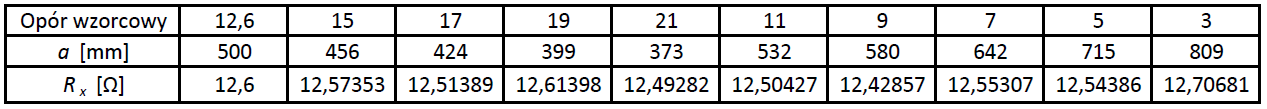
\includegraphics[width=\textwidth]{R1}
		\label{fig:r1}
	\end{figure}
	\begin{figure}[!h]
		\centering
		\caption{Pomiary oporu drugiego rezystora}
		%	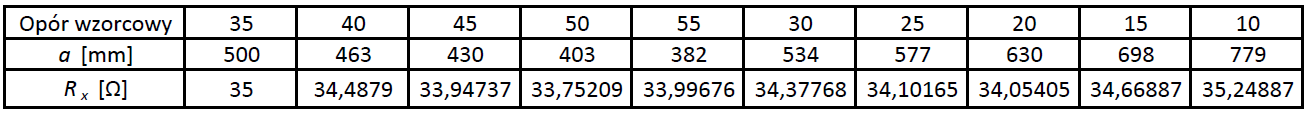
\includegraphics[width=\textwidth]{R2}
		\label{fig:r2}
	\end{figure}
	\begin{figure}[!h]
		\centering
		\caption{Pomiary oporu trzeciego rezystora}
	%	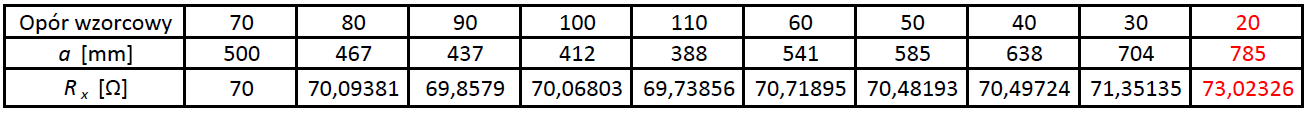
\includegraphics[width=\textwidth]{R3}
		\label{fig:r3}
	\end{figure}
	\begin{figure}[!h]
		\centering
		\caption{Pomiary oporu czwartego rezystora}
		%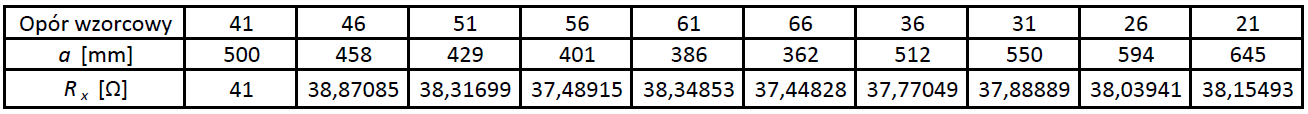
\includegraphics[width=\textwidth]{R4}
		\label{fig:r4}
	\end{figure}
	\begin{figure}[!h]
		\centering
		\caption{Pomiary oporu piątego rezystora}
	%	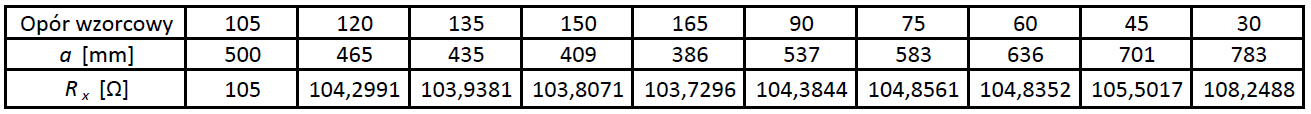
\includegraphics[width=\textwidth]{R5}
		\label{fig:r5}
	\end{figure}
	\begin{figure}[!h]
		\centering
		\caption{Pomiary oporu szeregowo podłączonych rezystorów 1 i 2}
		%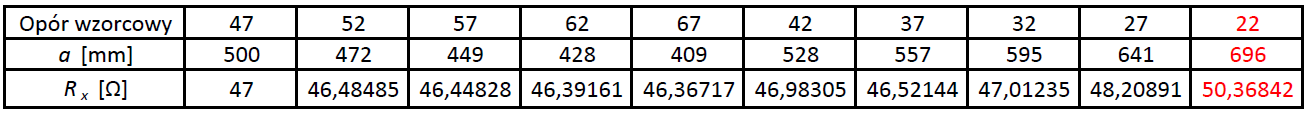
\includegraphics[width=\textwidth]{R1+R2}
		\label{fig:r1+r2}
	\end{figure}	
	\begin{figure}[!h]
		\centering
		\caption{Pomiary oporu równolegle podłączonych rezystorów 1 i 2}
	%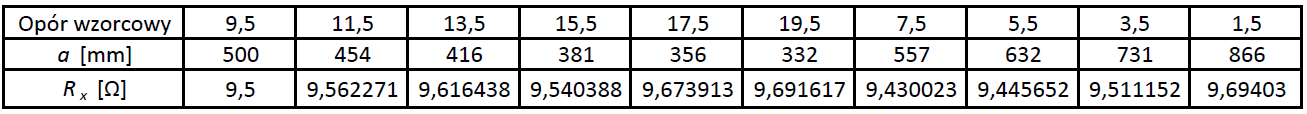
\includegraphics[width=\textwidth]{R1zR2}
		\label{fig:r1zr2}
	\end{figure}
	\begin{figure}[!h]
		\centering
		\begin{center}
		\caption{Pomiary oporu mieszanego połączenia rezystorów 1, 2 i 3}
	%	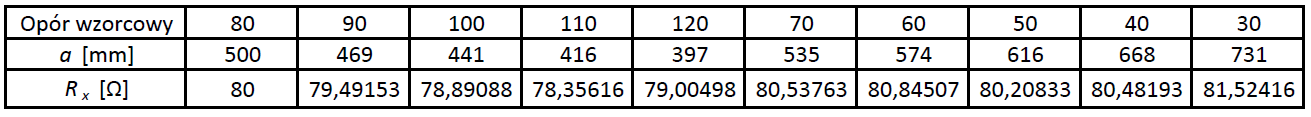
\includegraphics[width=\textwidth]{(R1zR2)+R3}
		\label{fig:(r1zr2)+r3}
		\end{center}
	\end{figure}
		
	

	\renewcommand*{\figurename}{Wykres} 
	\setcounter{figure}{0}
	\newpage
	\section{Opracowanie danych pomiarowych}\label{sec:opr}
	\subsection{Pomiary i ich niepewności.}
		
		Wszystkie pomiary wykonywaliśmy 10 razy dlatego przyjmujemy niepewność pomiaru typu A:
		
		Wyznaczone wartości rezystancji oporników i ich niepewności:
		\begin{itemize}
			\item $R_1=12,553$; $u(R_1)=0,024$
			\item $R_2=34,36$; $u(R_2)=0,15$
			\item $R_3=70,31$; $u(R_3)=0,15$
			\item $R_4=38,04$; $u(R_4)=0,13$
			\item $R_5=104,48$; $u(R_5)=0,18$
			\item $R_{z_1}=46,82$; $u(R_{z_1})=0,17$
			\item $R_{z_2}=9,567$; $u(R_{z_2})=0,031$
			\item $R_{z_3}=79,93$; $u(R_{z_3})=0,31$
		\end{itemize}	
 
	
	\subsection{Opracowanie danych.}\label{sec:drm}
	\begin{enumerate}[label=\alph*)]
		
		\item Analiza błędów.
		
		Stwierdzono wystąpienie błędów grubych, które wyraźnie odstają od średniej. Zaznaczono je w tabelkach kolorem czerwonym.
		
		\item Obliczenie wartości rezystancji połączeń szeregowego, równoległego i mieszanego korzystając z wyników pomiarów $R_1$, $R_2$ i $R_3$ i ich niepewności.
		
		Do policzenia wartości tych rezystancji wykorzystano następujące wzory: 
		\begin{equation}
		\label{eq:rz1}
		R_{z_1}=R_1 + R_2\text{,}
		\end{equation}
		\begin{equation}
		\label{eq:rz2}
		R_{z_2}=\frac{R_1 R_2}{R_1 + R_2}\text{,}
		\end{equation}
		\begin{equation}
		\label{eq:rz3}
		R_{z_3}=R_3 + \frac{R_1 R_2}{R_1 + R_2}\text{.}
		\end{equation}
		
		Niepewności wyliczenia rezystancji zastępczych obliczone zostały z wykorzystaniem prawa przenoszenia niepewności za pomocą następujących wzorów:
		\begin{equation}
		\label{eq:nrz1}
		u_c(R_{z_1})=\sqrt{\left[ u(R_1) \right]^2 + \left[ u(R_2) \right]^2}\text{,}
		\end{equation}
		\begin{equation}
		\label{eq:nrz2}
		u_c(R_{z_2})=\sqrt{\left[ \frac{R_2(2R_1+R_2)}{(R_1+R_2)^2} u(R_1) \right]^2 + \left[ \frac{R_1(2R_2+R_1)}{(R_1+R_2)^2} u(R_2) \right]^2}\text{,}
		\end{equation}
		\begin{equation}
		\label{eq:nrz3}
		u_c(R_{z_3})=\sqrt{\left[ u(R_3) \right]^2 + \left[ \frac{R_2(2R_1+R_2)}{(R_1+R_2)^2} u(R_1) \right]^2 + \left[ \frac{R_1(2R_2+R_1)}{(R_1+R_2)^2} u(R_2) \right]^2}\text{,}
		\end{equation}
		
		\item Otrzymano następujące wyniki:
		\begin{center}
			\begin{tabular}{|c|c|c|c|c|c|}
				\hline Opis wielkości & Opór wyznaczony $[\mathrm{\Omega}]$ & Opór obliczony $[\mathrm{\Omega}]$ & $u(R_x)$ $[\mathrm{\Omega}]$ & $u_c(R_x)$ $[\mathrm{\Omega}]$ \\
				\hline $R_{z_1}$ & 46,82 & 46,92 & 0,17 & 0,16  \\
				\hline $R_{z_2}$ & 9,567 & 9,194 & 0,031 & 0,075  \\  
				\hline $R_{z_3}$ & 79,93 & 79,51  & 0,31 &  0,17 \\ 
				\hline 
			\end{tabular} 
		\end{center}
		Można zauważyć, że wyniki dla połączenia szeregowego ($R_{z_1}$) i mieszanego ($R_{z_3}$) są zgodne w granicach wyznaczonych niepewności, lecz wynik połączenia równoległego ($R_{z_2}$) nie jest zgodny.
	
	\end{enumerate}
	
	\section{Podsumowanie}
	\begin{center}
		\begin{tabular}{|c|c|c|c|c|}
			\hline Opis wielkości & Opór wyznaczony $R_x$ $[\mathrm{\Omega}]$ & $u(R_x)$ $[\mathrm{\Omega}]$ &  $ \frac{u(R_x)}{R_x} $ $[\%]$ \\
			\hline $R_1$ & 12,553 & 0,024 & 0,19  \\
			\hline $R_2$ & 34,36 & 0,15 & 0,45  \\
			\hline $R_3$ & 70,31 & 0,15 & 0,21  \\
			\hline $R_4$ & 38,04 & 0,13 & 0,35  \\
			\hline $R_5$ & 104,48 & 0,18 & 0,17  \\
			\hline $R_{z_1}$ & 46,82 & 0,17 & 0,37  \\
			\hline $R_{z_2}$ & 9,567 & 0,031 & 0,33  \\  
			\hline $R_{z_3}$ & 79,93 & 0,31 & 0,39  \\ 
			\hline 
		\end{tabular} 
	\end{center}
\vspace{1em}

\begin{itemize}
	\item Mostek Wheatstone'a umożliwia mierzenie wartości oporu rezystorów, lub ich różnych połączeń. Pomiar ten jest dokładny nie uwzględniając spadków napięcia na przewodach służacych do odpowiedniego połączenia układu.
	\item Dzięki powtórzeniu pomiarów dla dziesięciu różnych ustawień opornicy dekadowej, udało się uzyskać bardzo dokładne wyniki, których błąd względny nie przekracza 0,5 \%. 
	\item Niezgodność porównania wartości obliczonej i wyznaczonej oporu rezystorów połaczonych równolegle może być spowodowana konieczością przebudowania układu pomiarowego (dodanie kolejnych przewodów, które posiadają swoją rezystancję).
	\item Błędy grube mogły być spowodowane przez przypadkowe przesunięcie kontaktu ślizgowego podczas odczytu wartości $a$ lub niedokładne wyzerowanie wskaźnika na mikroamperomierzu.
\end{itemize}

\end{document}